% ============================================================
% 第5章 问题2 模型建立与求解
% ============================================================

\section{模型建立与求解——问题2}

\subsection{矩形模型构建}
设第 $i$ 节板凳的两个把手中心分别为
\begin{equation}
P_i = (x_i, y_i), \qquad P_{i+1} = (x_{i+1}, y_{i+1}).
\end{equation}

定义板凳中心为
\begin{equation}
C_i = \frac{P_i + P_{i+1}}{2}.
\end{equation}

由两个把手确定板凳中心线方向，定义单位方向向量：
\begin{equation}
\mathbf{e}_i = \frac{P_{i+1} - P_i}{\|P_{i+1} - P_i\|}.
\end{equation}

其法向单位向量为：
\begin{equation}
\mathbf{n}_i = (-e_{iy}, e_{ix}).
\end{equation}

因此，第 $i$ 节板凳可以表示为：

以 $C_i$ 为中心、$\mathbf{e}_i$ 为纵向方向、长度为 $L_i$、宽度为 $w = 0.30\,\mathrm{m}$ 的矩形。

其中
\begin{equation}
L_i =
\begin{cases}
3.41, & i=1, \\[4pt]
2.20, & 2 \le i \le 222.
\end{cases}
\end{equation}

龙尾同样按照实际板长进行处理。
相邻把手距离明确：
\begin{equation*}
d_s = L_s - 2a = 2.20 - 2(0.275) = 1.65\,\mathrm{m}.
\end{equation*}

对于龙头：

\begin{equation*}
L_h = 3.41\,\mathrm{m},
\end{equation*}
\begin{equation*}
d_h = L_h - 2a = 3.41 - 2(0.275) = 2.86\,\mathrm{m}.
\end{equation*}




\subsection{分层碰撞检测}
对于全部$223$节板凳而言，全部直接进行逐一碰撞检测会十分复杂。因此，为了减少计算量和代码复杂度，我们引入分层碰撞检测的方法。

具体而言，我们按照顺序采用：

1. 角度筛选；

2. 圆距离筛选；

3. SAT精检。

\textbf{对于角度筛选}

由于舞龙队沿等距螺线向圆心方向盘入，相邻板凳的极角依次减小。

对于第 \(i\) 节板凳和其后第 \(j\) 节板凳，定义极角差为
\begin{equation*}
\Delta\theta_{ij} = \theta_i - \theta_j > 0.
\end{equation*}

由阿基米德螺线方程
\begin{equation*}
r = b\theta
\end{equation*}

可得两把手的径向距离差为
\begin{equation*}
|r_i - r_j| = b\Delta\theta_{ij}.
\end{equation*}

当
\begin{equation*}
\Delta\theta_{ij} > 3\pi
\end{equation*}

时，有
\begin{equation*}
|r_i - r_j| > 3\pi b = \frac{3p}{2} = 0.825\,\text{m}.
\end{equation*}

因此，随着极角差增大，两板凳在螺线上的空间间隔迅速增大。基于舞龙队的螺线排列结构，本文首先将
\begin{equation*}
0 < \Delta\theta_{ij} \leq 3\pi
\end{equation*}

范围内的板凳作为潜在碰撞对象，对超出该范围的板凳对进行预筛除，以减少后续碰撞检测的计算量。

\textbf{对于圆距离筛选}

为进一步降低矩形精确碰撞检测的计算量，将每节板凳矩形用其外接圆进行包络。

设第 \(i\) 节板凳的中心为 \(C_i\)，长度为 \(L_i\)，宽度为 \(w\)，则其外接圆半径为
\begin{equation*}
R_i = \frac{1}{2}\sqrt{L_i^2 + w^2}.
\end{equation*}

由于板凳矩形完全包含于其外接圆内，因此若两节板凳发生碰撞，则其外接圆必然相交。故由逆否命题可得：
\begin{equation*}
\|C_i - C_j\| > R_i + R_j \Rightarrow \text{板凳 } i, j \text{ 不发生碰撞.}
\end{equation*}

因此，在进行矩形精确碰撞检测前，首先计算两板凳中心之间的距离。若满足上述条件，则直接判定两板凳不存在碰撞，无需进一步进行分离轴定理检测；只有当：
\begin{equation*}
\|C_i - C_j\| \leq R_i + R_j
\end{equation*}

时，才将该板凳对纳入后续的矩形精确碰撞判定。

\subsection{基于 SAT 的精确碰撞判定}

由于相邻板凳本身通过把手连接，因此本文主要判断非相邻板凳之间是否发生碰撞，即当：

\begin{equation*}
|i-j| \ge 2.
\end{equation*}

对于任意两节非相邻板凳 $i,j$，采用分离轴定理（Separating Axis Theorem，SAT）进行矩形相交判定。下面先引入分离轴定理。

分离轴（SAT）定理：对于两个凸矩形，如果存在一条直线方向，使得两个矩形在该方向上的投影区间互不重叠，则两矩形不发生碰撞。

特别地：对于两个矩形，只需考察它们自身的边方向及其法向方向。因此选取以下四个候选方向：
\begin{equation*}
u \in \{ e_i, n_i, e_j, n_j \}.
\end{equation*}


设矩形 \(i\) 的中心为 \(C_i\)，长度为 \(L_i\)，宽度为 \(w\)。

在任意单位方向 \(\mathbf{u}\) 上，其投影半径为：
\begin{equation*}
R_i(\mathbf{u}) = \frac{L_i}{2}|\mathbf{e}_i \cdot \mathbf{u}| + \frac{w}{2}|\mathbf{n}_i \cdot \mathbf{u}|.
\end{equation*}

因此矩形 \(i\) 在 \(\mathbf{u}\) 方向上的投影区间为：
\begin{equation*}
I_i(\mathbf{u}) = [C_i \cdot \mathbf{u} - R_i(\mathbf{u}), C_i \cdot \mathbf{u} + R_i(\mathbf{u})].
\end{equation*}

矩形 \(j\) 同理。

两个矩形在方向 \(\mathbf{u}\) 上发生投影分离，当且仅当：
\begin{equation*}
|(C_i - C_j) \cdot \mathbf{u}| > R_i(\mathbf{u}) + R_j(\mathbf{u}).
\end{equation*}

若对于四个候选方向中的任意一个方向均满足上述不等式，则两个矩形存在分离轴，因此：
板凳 \(i,j\) 不发生碰撞。

反之，如果四个方向均不存在投影分离，即：
\begin{equation*}
|(C_i - C_j) \cdot \mathbf{u}| \leq R_i(\mathbf{u}) + R_j(\mathbf{u}), \quad \forall \mathbf{u} \in \{\mathbf{e}_i, \mathbf{n}_i, \mathbf{e}_j, \mathbf{n}_j\}.
\end{equation*}

则认为两节板凳发生碰撞。

\subsection{首次碰撞时刻的确定}
我们首先定义碰撞状态函数
\begin{equation*}
C(t) = \begin{cases} 0, & \text{时刻 } t \text{ 无板凳碰撞}, \\ 1, & \text{时刻 } t \text{ 存在板凳碰撞}. \end{cases}
\end{equation*}

首次碰撞时刻定义为
\begin{equation*}
t^* = \inf\{t : C(t) = 1\}.
\end{equation*}

首先以一定时间步长对盘入过程进行粗搜索，并在各时刻依次进行“极角范围粗筛—外接圆粗筛—SAT精确判定”，确定满足
\begin{equation*}
C(t_k) = 0, \quad C(t_{k+1}) = 1
\end{equation*}

的时间区间，即
\begin{equation*}
t^* \in [t_k, t_{k+1}].
\end{equation*}

随后沿用问题一中的二分法，在该区间内取
\begin{equation*}
t_m = \frac{t_L + t_R}{2},
\end{equation*}

根据碰撞状态不断缩小搜索区间，直至
\begin{equation*}
|t_R - t_L| < \varepsilon_t.
\end{equation*}

最终取
\begin{equation*}
t^* = \frac{t_L + t_R}{2}
\end{equation*}

作为板凳龙首次发生碰撞的临界时刻。

经计算，板凳龙首次发生碰撞的时间为412.47s。
\begin{figure}[htbp]      
    \centering              % 图片居中
    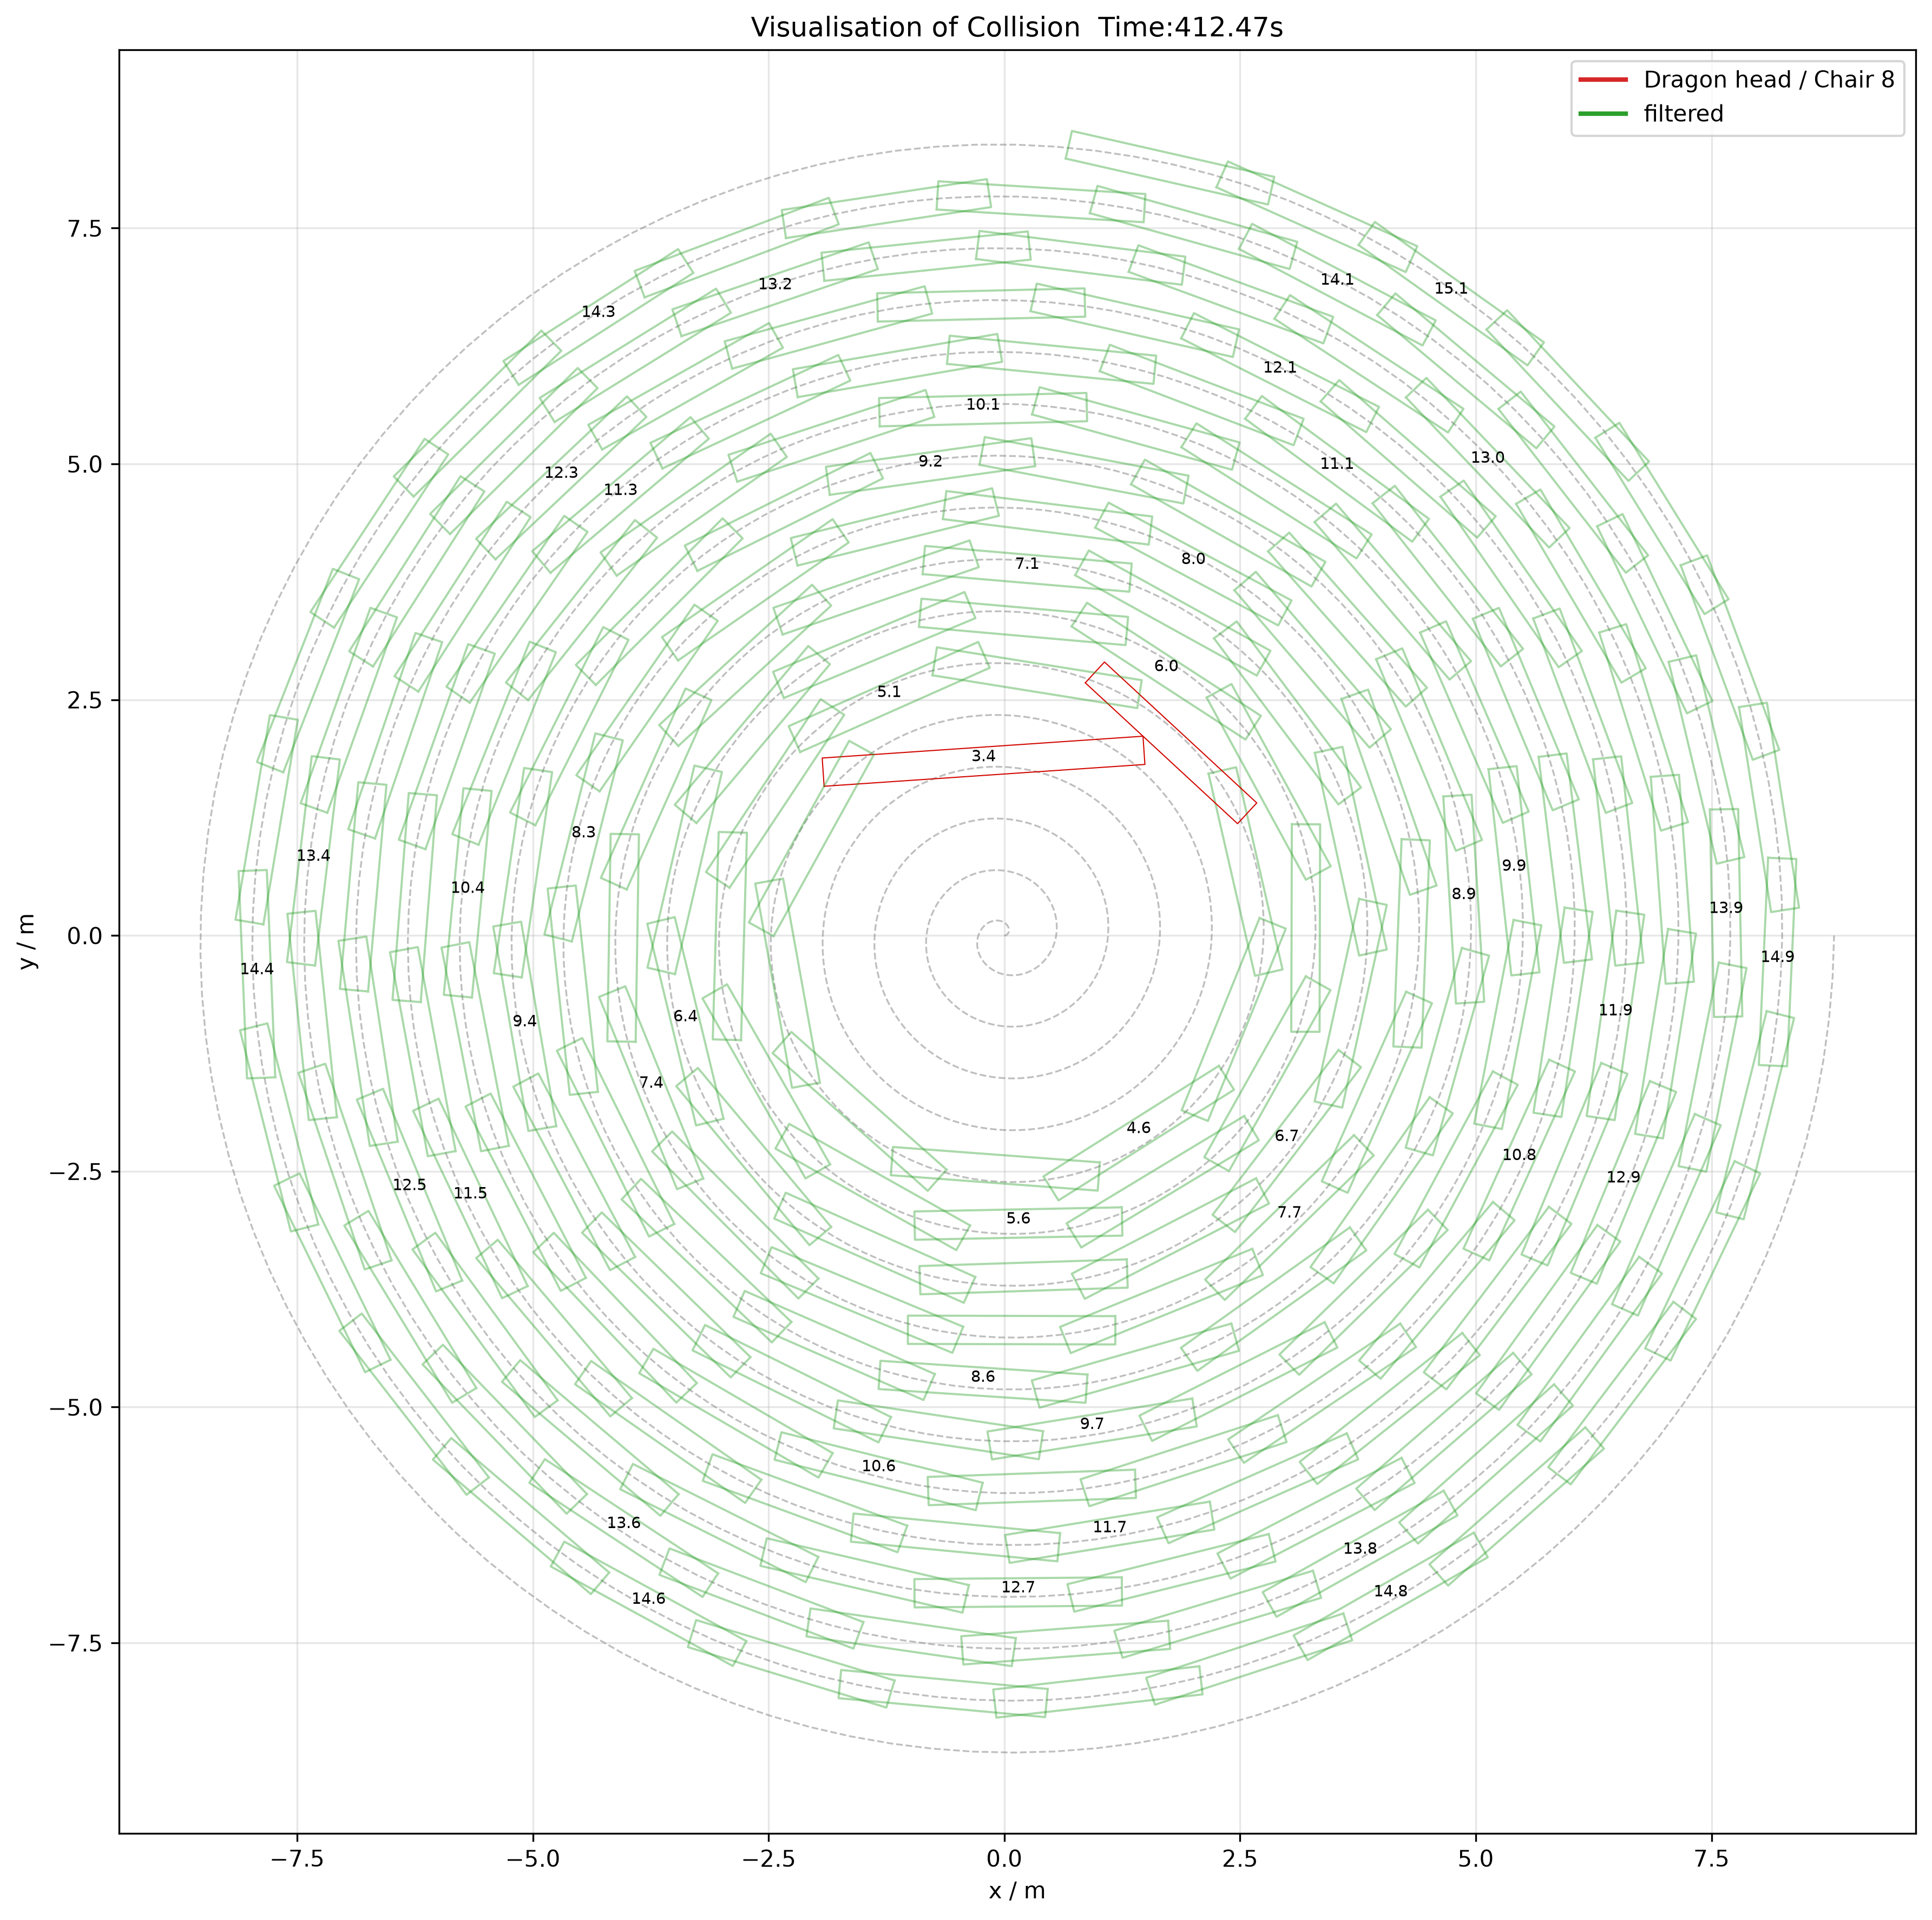
\includegraphics[width=0.8\textwidth]{images/碰撞图 412.47.png} % 插入图片
    \caption{碰撞时刻示意图} % 图片标题
    \label{fig:third}     % 标签，用于引用
\end{figure}



\subsection{各把手的位置和速度的求解}
确定首次碰撞的临界时刻 \(t^*\) 后，利用问题一中的把手位置递推模型求得各把手极角 \(\theta_i(t^*)\)。将其代入阿基米德螺线参数方程，可得各把手位置
\begin{equation*}
P_i(t^*) = (b\theta_i(t^*)\cos\theta_i(t^*), b\theta_i(t^*)\sin\theta_i(t^*)).
\end{equation*}

对位置方程关于时间求导，得到
\begin{equation*}
\dot{x}_i = b(\cos\theta_i - \theta_i\sin\theta_i)\dot{\theta}_i,
\end{equation*}
\begin{equation*}
\dot{y}_i = b(\sin\theta_i + \theta_i\cos\theta_i)\dot{\theta}_i.
\end{equation*}

又由螺线弧长关系
\begin{equation*}
\frac{ds}{d\theta_i} = b\sqrt{1+\theta_i^2}, \quad \frac{ds}{dt} = v,
\end{equation*}

可得
\begin{equation*}
\dot{\theta}_i = \frac{v}{b\sqrt{1+\theta_i^2}}.
\end{equation*}

因此各把手速度大小为
\begin{equation*}
v_i = \sqrt{\dot{x}_i^2 + \dot{y}_i^2} = v.
\end{equation*}


